\documentclass[12pt,oneside]{book}
\newcommand{\TITLE}{Basics Quantum Physics}
\usepackage[utf8]{inputenc}
\usepackage[margin=0.5in]{geometry}
\usepackage[usestackEOL]{stackengine}
\usepackage{amsmath , esint,braket,lmodern,mhchem,bohr,lewis,chemfig,draftwatermark,xcolor,graphicx , amssymb ,ragged2e , listings , siunitx , float , eqparbox, centernot , esvect , bm , fancyhdr , fourier-orns}
\usepackage[ddmmyyyy]{datetime}
\usepackage{fourier-orns}
\usepackage{changepage}
\usepackage{bbm}\usepackage{chngcntr}
\usepackage{hyperref}
\usepackage{ifthen}
\usepackage[many]{tcolorbox}
\DeclareMathOperator{\sech}{sech}
\DeclareMathOperator{\csch}{csch}
\DeclareMathOperator{\arcsec}{arcsec}
\DeclareMathOperator{\arccot}{arcCot}
\DeclareMathOperator{\arccsc}{arcCsc}
\DeclareMathOperator{\arccosh}{arcCosh}
\DeclareMathOperator{\arcsinh}{arcsinh}
\DeclareMathOperator{\arctanh}{arctanh}
\DeclareMathOperator{\arcsech}{arcsech}
\DeclareMathOperator{\arccsch}{arcCsch}
\DeclareMathOperator{\arccoth}{arcCoth} 
\DeclareMathOperator{\grad}{\vv{\text{grad}}} 
\DeclareMathOperator{\conj}{^*} 
\DeclareMathOperator{\vect}{vv} 
\DeclareMathOperator{\Vect}{\text{Vect}} 
\DeclareMathOperator{\degree}{c^\circ} 
\DeclareMathOperator{\degre}{^\circ} 
\DeclareMathOperator{\transpose}{^\dagger} 
\DeclareMathOperator{\adjoint}{^\dagger} 

\newcommand{\moyenne}[1]{\langle #1 \rangle} 
\newcommand{\lagrange}{\mathcal{L}}
\newcommand{\fourier}{\mathcal{F}}
\newcommand{\hilbert}{\mathcal{H}}
\newcommand{\p}{\mathcal{P}}
\newcommand{\x}{\chi}
\newcommand{\ve}[1]{\vv{#1}}
\newcommand{\push}[1]{\begin{adjustwidth}{5mm}{}#1\end{adjustwidth}}
\newcommand{\operator}[1]{\widehat{#1}}
\newcommand{\HRule}{\rule{\linewidth}{0.5mm}} % Defines a new command for the horizontal lines, change thickness here
\renewcommand{\chaptermark}[1]{\markboth{\MakeUppercase{#1}}{}}
\renewcommand{\headrule}{%
\vspace{-8pt}\hrulefill
\raisebox{-2.1pt}{\quad\decofourleft\decotwo\decofourright\quad}\hrulefill}
\definecolor{myred}{RGB}{255, 14, 0}
\everymath{\displaystyle}

\def\changemargin#1{\list{}{\leftmargin#1}\item[]}
\let\endchangemargin=\endlist 

\makeatletter
\newcommand*{\rom}[1]{\expandafter\@slowromancap\romannumeral #1@}%roman numbers
\makeatother

%hyperlink shit

\hypersetup{
    colorlinks,
    citecolor=black,
    filecolor=black,
    linkcolor=black,
    urlcolor=black
}
% Table specail cell , it's for making line break in table cell
\newcommand{\specialcell}[2][c]{%
  \begin{tabular}[#1]{@{}c@{}}#2\end{tabular}}

  \definecolor{main}{HTML}{5989cf}    % setting main color to be used
\definecolor{sub}{HTML}{cde4ff}     % setting sub color to be used

\tcbset{
    sharp corners,
    colback = white,
    before skip = 0.2cm,    % add extra space before the box
    after skip = 0.5cm      % add extra space after the box
}   
\newtcolorbox{boxH}{
    colback = sub, 
    colframe = main, 
    boxrule = 0pt, 
    leftrule = 6pt % left rule weight
}
\newtcolorbox{gpt}{
    sharpish corners, % better drop shadow
    boxrule = 0pt,
    toprule = 4.5pt, % top rule weight
    enhanced,
    fuzzy shadow = {0pt}{-2pt}{-0.5pt}{0.5pt}{black!35} % {xshift}{yshift}{offset}{step}{options} 
}
\definecolor{codegreen}{rgb}{0,0.6,0}
\definecolor{codegray}{rgb}{0.5,0.5,0.5}
\definecolor{codepurple}{rgb}{0.58,0,0.82}
\definecolor{backcolour}{rgb}{0.95,0.95,0.92}

\lstdefinestyle{mystyle}{
    backgroundcolor=\color{backcolour},   
    commentstyle=\color{codegreen},
    keywordstyle=\color{magenta},
    numberstyle=\tiny\color{codegray},
    stringstyle=\color{codepurple},
    basicstyle=\ttfamily\footnotesize,
    breakatwhitespace=false,         
    breaklines=true,                 
    captionpos=b,                    
    keepspaces=true,                 
    numbers=left,                    
    numbersep=5pt,                  
    showspaces=false,                
    showstringspaces=false,
    showtabs=false,                  
    tabsize=2,
    basicstyle = \small
}

\lstset{style=mystyle}
\SetWatermarkAngle{45} 
\SetWatermarkLightness{.99} 
\SetWatermarkFontSize{0.1cm} 
\SetWatermarkScale{0} 
\SetWatermarkText{supahaka}


\begin{document}
\pagestyle{fancy}
\fancyhf{}
\fancyfoot[R]{Tenji$_\text{org}$}
\fancyfoot[C]{\thepage}
\fancyfoot[L]{\tiny www.tenji.org}
\fancyhead[RO]{\nouppercase{\leftmark\hfill\TITLE}}


\DraftwatermarkOptions{stamp=false}
    \begin{titlepage}
        \begin{center}
            \vspace*{5cm}
            \Huge
            \HRule \\[0.4cm]
            \textbf{Project Tenji: \\ \TITLE}\\
            \Large 
            \HRule \\[1.5cm]
            \vspace{2cm}
            \vfill
        \end{center}
        \vfill
        { \scriptsize Project Tenji \copyright 2024 by Khalil Salahat and Mohamad El Moussawi  \\}
        { \scriptsize Hosted at tenji.org , contact : contact@tenji.org \\}
        { \scriptsize \NOTICEE  \\}
    \end{titlepage} 
    \tableofcontents
\DraftwatermarkOptions{stamp=true}

\chapter{Quantum Mechanics Postulates}
\section{Definition}
Quantum mechanics for us is a set of rules to allow us to make predictions about the world and these rules will be awesome if their predictions are good,and if their prediction are bad, these rules will suck.\\
We will avoid bad rules to the degree possible.
\begin{center}
	We will get what we've learned over the past 100 year of developing QUANTUM MECHANICS
\end{center}
\section{Postulate \rom{1}}
The state of a Quantum object is completely specified by a single function (wave function) $\psi(x)$ , which is a complex function.
\section{Postulate \rom{2}}
\begin{itemize}
	\item The probability that upon measurement the object found on the position x is equal to $|\psi(x)|^2$ \\
	      \[\p(x) = |\psi(x)|^2\]
	      \begin{center}
		      ($\p(x) $ determines probability density that the object in state $\psi$ will be found at x.)
	      \end{center}
	      \[ \p(x,x+dx) = \p(x)dx = |\psi(x)|^2dx \]
	\item Total probability that you find something somewhere must be 1 :
	      \[ \int_\text{All} dx \p(x) = 1 \]
	\item Normalization :\\
	      The probabilities must always be normalized $ \int^{+\infty}_{-\infty} dx |\psi(x)|^2 = 1$.
	      \begin{center}
		      \underline{Normalization is the scaling of wave functions so that all the probabilities add to 1.}
	      \end{center}
\end{itemize}
\subsection{Probabilities visualization}
Now consider the following wave functions $\psi(x)$ and their probabilities $\p(x)$ :
\begin{itemize}
	\item \begin{minipage}{0.3\linewidth}
		      $\psi(x)$\\
		      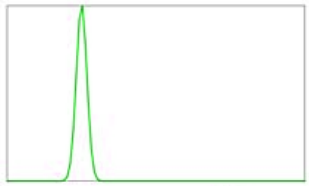
\includegraphics[width=\linewidth]{../pic/3302/6.png}\\
	      \end{minipage}
	      \begin{minipage}{0.3\linewidth}
		      $\p(x)$\\
		      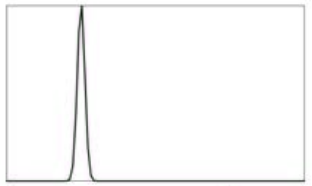
\includegraphics[width=\linewidth]{../pic/3302/7.png}
	      \end{minipage} \\
	      \begin{itemize}
		      \item  We can see that $x$ is determined, and its uncertainty $\Delta x $ is small.
		      \item And $p$ is not determined, and its uncertainty $\Delta p$ is large.\\
		            That's because there is no clear wave length for it, it's not periodic, and as DeBroglie said if you have a definite wave length, you have a definite momentum ($P= \hbar k$)
	      \end{itemize}
	      \item\begin{minipage}{0.3\linewidth}
		      $\psi(x)$ \\
		      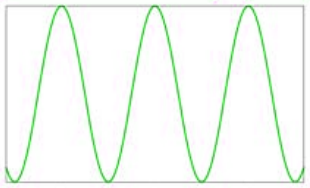
\includegraphics[width=\linewidth]{../pic/3302/10.png}\\
	      \end{minipage}
	      \begin{minipage}{0.3\linewidth}
		      $\p(x)$\\
		      
\includegraphics[width=\linewidth]{../pic/3302/11.png}
	      \end{minipage}\\
	      Here we have the equation of the wave function as following: $\psi = - e^{ik_1x}$ \\
	      The probability $\p(x) = |e^{i\alpha}|^2 = 1 ;( \text{ remember : }e^{-i\alpha} = (e^{i\alpha})\conj$)
	      \begin{itemize}
		      \item So here $x$ is not determined ($\p(x) =1 $ over all of x), and its uncertainty $\Delta x $ is very large.
		      \item In the other hand this exactly a periodic function with determined wavelength $\lambda_1 = \frac{ 2\pi}{k_1}$ , with $P = \hbar k_1$ we can say that the momentum is determined, and its uncertainty $\Delta P $ is  small\\
	      \end{itemize}
\end{itemize}

\section{Postulate \rom{3}}
This is the most important thing in all of quantum mechanics, it is all contained in the following proposition:\\
Given two possible wave function (configuration) of a quantum system corresponding to two distinct wave function $\psi_1(x)$ and $\psi_2(x)$ , the system can \underline{also} be in a \underline{superposition}  of $\psi_1(x)$ and $\psi_2(x)$ :
\[\boxed{\psi(x) = \alpha\psi_1(x) + \beta\psi_2(x)}\]
Where $\alpha$ and $\beta$ are complex numbers subjects to the normalization condition.
\begin{center}
	(Given any two possible configurations of the system, there is also an allowed configuration of the system corresponding to being in an arbitrary superposition of them.)\\
	This forms the soul of quantum mechanics
\end{center}
\subsection{Consequences}
\begin{itemize}
	\item Any reasonable function $\psi(x)$ can be expressed as a superposition of more easily interpretable wave functions.
	      \begin{itemize}
		      \item Any function can be expressed as a superposition of  states (wave functions)  with a definite momentum:
		            \[ \psi(x) = \frac{1}{\sqrt{2\pi}}\int dk \widehat{\psi}(k)e^{ikx} \]
		      \item Any function can be expressed as a superposition of states (wave functions) with definite position:
		            \[ \psi(x) = \int dx_0 \psi(x_0)\delta(x-x_0) \]
	      \end{itemize}
	\item The probability density
	      \[ \p(x) = |\alpha\psi_a(x) + \beta\psi_b(x)|^2 = \underbrace{|\alpha \psi_a(x)|^2+|\beta\psi_b(x)|^2}_{\p_1 + \p_2}+\underbrace{\alpha\conj\beta\psi_a\conj(x)\psi_b(x) + \alpha\beta\conj\psi_a(x)\psi_b(x)\conj}_\text{interference terms} \]
\end{itemize}
\subsection{Transform Momentum-Position}
\begin{center}
	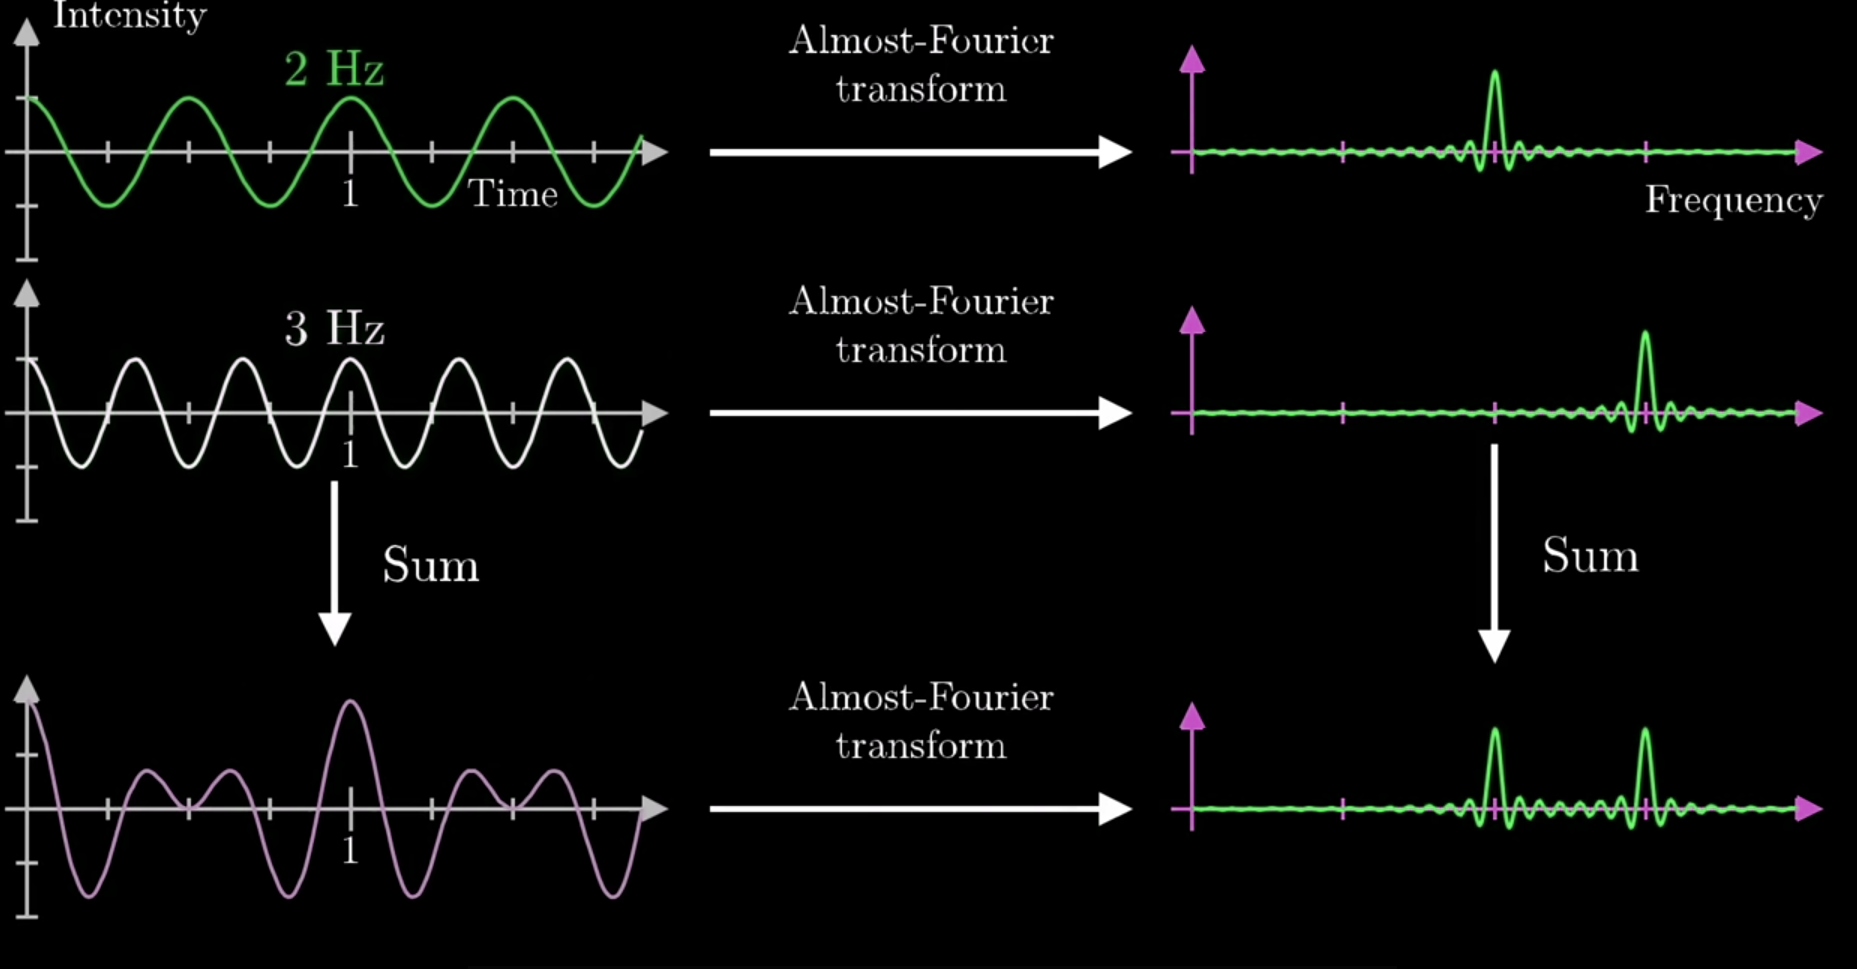
\includegraphics[width=0.7\linewidth]{../pic/3302/14.png}
\end{center}
Fourier Transform :
\[  \boxed{f(x) = \frac{1}{\sqrt{2\pi}}\int^{+\infty}_{-\infty}dk \widetilde{f}(k)e^{ikx}}   \]
The Inverse Fourier Transform :
\[ \boxed{\widetilde{f}(k)=\frac{1}{\sqrt{2\pi}} \int^{+\infty}_{-\infty} dx f(x e^{-ikx})} \]
So note that there is a sort of pleasing symmetry here :
\begin{center}
	\begin{itemize}
		\item If your wave function is well localized, corresponding to a reasonably \underline{well-defined position},\\then your \underline{Fourier transform is not well localized}, corresponding to \underline{not having a definite momentum}.
		\item On the other hand, if you have \underline{definite momentum}, your \underline{position is not well-defined},\\but the \underline{Fourier transform has a single peak} at the value of k corresponding to the momentum of your wave.
	\end{itemize}
\end{center}
\section{Average, Uncertainty}
Given that, the system is in a state described by the wave function $\psi(x)$.\\
\push{
	the average position value is :
	\[ \moyenne{x}_\psi=  \int^{+\infty}_{-\infty}dx |\psi(x)|^2 x\]
	and similarly for any function of x :
	\[\moyenne{f(x)}_\psi =  \int^{+\infty}_{-\infty}dx|\psi(x)|^2f(x) \]
	The position uncertainty :
	\[\Delta x^2 =  \moyenne{x^2}_\psi-\moyenne{x}_\psi^2 \]
	Note that the notation $\moyenne{x}_\psi = \braket{\psi|x|\psi}$\\
}
Given that, the system is in a state described by the wave function $\psi(p)$.\\
\push{the average momentum value is :
	\[ \moyenne{p}_\psi=  \int^{+\infty}_{-\infty}dp \underbrace{|\psi(p)|^2}p\]
	for any function of p :
	\[\moyenne{f(p)}_\psi =  \int^{+\infty}_{-\infty}dx|\psi(p)|^2f(p) \]
	The Momentum uncertainty :
	\[\Delta p^2 =  \moyenne{p^2}_\psi-\moyenne{p}_\psi^2 \]}
\section{Operators}
\subsection{Definition}
\begin{itemize}
	\item Operators are some instruction that act on objects and scramble them.
	\item The operators act on the object and gives another object.
\end{itemize}
The simplest model in mathematics to describe the operators are the matrices, and for the objects are the vectors.\\
In Quantum Mechanics, the objects are a complex function of x, and the operators act on the functions.\\
\subsection{Linear Operator}
\begin{center}
	A linear operator is an operator that respect superposition.
\end{center}
$\widehat{\theta}$ is a linear operator if :
\[\widehat{\theta}(af(x)+bf(x)) = a\widehat{\theta}f(x) + b\widehat{\theta}g(x )\]
\subsection{Eigenvectors}
If you have a given matrix m, there are some vectors that acted by n remain the same direction, they may grow a little or become smaller, but they remain in the same direction.\\
These are called eigenvectors, and that constant of proportionality, proportional to the action of the operator on the vector, is called the eigenvalue.\\
So operators can have eigenfunction, let us consider the following linear operator :
\[\hat{A}f_a(x) = af(x)\begin{cases}
		a : \text{The eigenvalue.} \\
		f(x): \text{the eigenfunction}
	\end{cases}\]
Example : \\
\push{
$\hat{A} = \hat{p}\begin{cases}
		e^{ikx} : \text{is the eignfunction} \\
		\hbar : \text{is the eignvalue}
	\end{cases}$\\
because $\hat{p}e^{ikx} = \hbar k e^{ikx}$
}
\subsection{Momentum operator }
We know that : having a wave with wave number k or  wavelength lambda $k=\frac{2\pi}{\lambda }$ is associated with momentum : $p=\hbar k$.\\
But in particular a plane wave with wavelength $\lambda$ look like $e^{ikx}$, how do i get $\hbar k$ out of it ?\\
$\underbrace{\frac{\partial}{\partial x}e^{ikx}} = ike^{ikx}$, so i can multiply by $\frac{\hbar}{i}\frac{\partial}{\partial x}e^{ikx} = \hbar k e^{ikx} = \underbrace{pe^{ikx}} \\
	\implies \frac{\hbar}{i}\frac{\partial}{\partial x} = p$ \\
Well, that deeply unsatisfying, so
\begin{center}
	What does momentum have to do with a derivative ?
\end{center}
\subsubsection{Noether's theorem}
To every continuous symmetry is associated a conserved quantity :
\begin{itemize}
	\item For translation symmetries $x\to x+L$ : Conservation of momentum $\dot{p} = 0$
	\item For time translation symmetries$t \to t + T$ : Conservation of Energy $\dot{E} = 0$
	\item For rotation symmetries $ \vv{x} \to \vv{\mathcal{R}x} $ : Conservation of Angular momentum $\dot{\vv{L}} = 0$
\end{itemize}
\subsubsection{$\frac{\partial }{\partial x}$ and translation}
$T_L :$ is the translation operator defined as $T_Lf(x) = f(x-L)$.\\
If we apply Taylor expansion, we got :\\
\begin{align*}
	T_Lf(x) & = f(x-L)                                                                                                                                                                                                        \\
	        & =f(x) - L\frac{\partial}{\partial x}f(x)+ \frac{L^2}{2}\frac{\partial^2}{\partial x^2}f(x)...                                                                                                                   \\
	        & =\underbrace{(1-L\frac{\partial}{\partial x} + \frac{L^2}{2}\frac{\partial^2}{\partial x^2} - \frac{L^3}{5}\frac{\partial^3}{\partial x^3})}_\text{Taylor expansion of $e^{-\frac{L\partial}{\partial x}}$}f(x) \\
	        & =e^{-L\frac{\partial}{\partial x}}f(x)                                                                                                                                                                          \\
	        & \implies T_L = e^{-L\frac{\partial}{\partial x}}
\end{align*}
If $L$ is small $\implies$ $T_L = f(x) - L \frac{\partial}{\partial x}f(x)$ , so we can say that $\frac{\partial}{\partial x}$ generates small translations in x.
\subsubsection{Relation $\frac{\partial}{\partial x}$ -- $p$}
\begin{itemize}
	\item Translation in x are generated by $\frac{\partial}{\partial x}$
	\item Noether's theorem : Translation in x are associated with conservation of momentum
\end{itemize}
\begin{center}
	So it's not totally shocking that in Quantum Mechanics $\frac{\partial}{\partial x}$ is associated with the momentum,  and more $\frac{\partial}{\partial t} $ associated with the energy
\end{center}
\subsection{Observable operators}
To each observable, we have an associated operator :\\
$\hat{A} = \begin{cases}
		\text{Momuntum : } \hat{p} = \frac{\hbar}{i}\frac{\partial}{\partial x} \\
		\text{Position : } \hat{x} = x                                          \\
		\text{Energy : } \hat{E} = \frac{\hat{p}}{2m}+ V(\hat{x}) = -\frac{\hbar^2}{2m}\frac{\partial^2}{\partial x^2} + V(\hat{x})
	\end{cases}$\\
The expectation value : $\moyenne{\hat{A}} = \int dx \psi(x)\conj\hat{A}\psi(x)$\\
The uncertainty : $(\Delta A)_\psi = \sqrt{\moyenne{\hat{A}^2}-\moyenne{A}^2}$
\subsection{Commutator}
The commutator of two operators quantifies how well the two observable described by these operators can be measured simultaneously.
\[ [\hat{A},\hat{B}] = \hat{A}\hat{B}-\hat{B}\hat{A} \]
\subsubsection{Commutator and Eigenfunction}
	Consider $\hat{A},\hat{B}$ Where $\hat{A}\psi_{ab} = a\psi_{ab}$ and $\hat{B}\psi_{ab} = b\psi_{ab}$ ,$\hat{A}$ and $\hat{B}$ have the same eigenfunction.\\
	$[\hat{A},\hat{B}]\phi_{ab} = (AB-BA)\phi_{ab} = AB\phi_{ab}-BA\phi_{ab} = a(b\phi_{ab})-b(a\phi_{ab}) = 0$.
	\begin{center}
		So in order fo $\hat{A}$ and $\hat{B}$ to share a single eigenfunction $\phi_{ab}$, the commutator must annihilate that particular common eigenfunction.
	\end{center}
	Now Consider $[\hat{A},\hat{B}] = c \mathbbm{1}$\\
	Those operators can't share any eigenfunction because $\mathbbm{1}$ doesn't annihilate any wave function, nothing is 0 when acted upon by the identity.\\
	Now in term of observables :\\
	if $\hat{A}$ and $\hat{B}$ are two observables and their commutator is proportional to the identity
	\begin{center}
		It is impossible for a state exist with a definite value of $\hat{A}$ and definite value of $\hat{B}$ simultaneously.
	\end{center}
	And we can say about the uncertainty :
	\[\boxed{\Delta A_\psi\Delta_\psi B \geq \frac{1}{2} |\braket{\psi|[A,B]|\psi}|}\]
\subsubsection{Momentum--Position commutation :}
$[\hat{x},\hat{p}] = ?$ \\
$ (\hat{p}\hat{x})f(x) = \hat{p}(\hat{x}f(x))= \hat{p}(xf(x)) = \frac{\hbar}{i}\frac{\partial}{\partial x}(xf(x)) = \frac{\hbar}{i}f(x) + \frac{\hbar}{i}x\frac{\partial f}{\partial x}\\$
$(\hat{x}\hat{p})f(x) = \hat{x}(\hat{p}f(x)) = \hat{x}(\frac{\hbar}{i}\frac{\partial f}{\partial x}) = \frac{\hbar}{i}\times \frac{\partial f}{\partial x}$\\
$(\hat{x}\hat{p}-\hat{p}\hat{x})f(x) = - \frac{\hbar}{i}f(x) = i\hbar f(x) \\$
$[\hat{x},\hat{p}]f(x) = i\hbar f(x) \implies \boxed{[\hat{x},\hat{p}] = \mathbbm{1}i\hbar}$\\
\begin{center}
	It is impossible for a state exist with a definite value of momentum and definite value of position simultaneously.
\end{center}
And so we can say : 
\[\boxed{\Delta x\Delta p \geq \frac{\hbar}{2}}\]

\subsection{Hermitian adjoint}
Given any linear operator $\hat{\theta}$, we can build $\hat{\theta}\transpose$ : \\
\[\boxed{\int dxf\conj(\hat{\theta}\transpose g) = \int dx(\hat{\theta}f)\conj g}\]
we call $\hat{\theta}\transpose$ Adjoint (Hermitian adjoint) of $\hat{\theta}$
\begin{itemize}
	\item Example 1 : $C$ is a complex number what is $C\adjoint$? \\
	      $ \underbrace{\int dx f\conj(C\adjoint g) } = \int dx( f)\conj g  = \underbrace{\int dx f\conj (\conj g)} \implies \boxed{C\adjoint = C\conj} $
	\item Example 2 : What is $\partial_x\adjoint$ acting on \underline{Normalizable function} \\
	      Note : ($\partial_x$ is the derivate with respect to x operator $\frac{d}{dx}$)\\
	      $\underbrace{\int dx f\conj(\partial_x\adjoint g)} = \int dx (\partial_x f)\conj g= \int dx (\partial_x f\conj)g = -\int dx f\conj \partial_x g = \underbrace{\int dx f\conj(-\partial_x g)} \implies \boxed{\partial_x\adjoint = - \partial_x}$
	\item Example 3 : What $\hat{X}\adjoint$ \\
	      $\int dx f\conj(\hat{x}\adjoint g) = \int dx (\hat{x}f)\conj g = \int dx x f\conj g = \int dx f\conj (xg) \implies \boxed{\hat{x}\adjoint = \hat{x}} $
\end{itemize}
\subsection{Hermitian Operator}
An operator $\hat{\theta}$ where $\hat{\theta}\adjoint = \hat{\theta} $ is hermitian.\\
Note :
\begin{itemize}
	\item A hermitian number is real.
	\item A hermitian operator, his eigenvalue is real.
	\item All the observable are real, all the observable operators must be hermitian operators.
	\item $(AB)\adjoint = B\adjoint A\adjoint$
\end{itemize}

\section{Postulate \rom{3} -- Superposition with operators}
\[\boxed{\psi(x) = \sum_a C_a\psi_a(x)}\]
Given an observable $\hat{A}$ , and its eigenfunction, $\phi_a(x)$ One can expand $\psi$ as:
\begin{center}
	Any state can  be written as superposition of $\sum_a C_a\psi_a(x)$
\end{center}
Example:\\
\push{
	$\psi(x)$ an arbitrry funciton
	\begin{itemize}
		\item We can write $\psi(x)$ as a superposition (with some coefficients $\psi(x_0)$) of states with \underline{definite position}:\\
		      $\psi(x) = \int dx_0\delta(x-x_0)\psi(x_0) $
		\item We can do the same for momentum eigenfunction, any function can be expanded in a superposition of \underline{momentum eigenfunction} (with some coefficients $\widetilde{\psi}(k)$):\\
		      $\psi(x) = \int dk \frac{1}{\sqrt{2\pi}}e^{ikx}\widetilde{\psi}(k)$
		\item Any wave function can be expanded in states with \underline{energy eigenfunction} (with some coefficient $C_n$):\\
		      $\psi(x)  = \sum_n\phi_n(x)C_n$
	\end{itemize}
}
We are going to harp on energy eigenfunction because they're more convenient for solving the time evolution problem :
\push{
The Shrodinger equation : $i\hbar \partial_t\psi(x,t) = \hat{E}\psi(x,t)$\\
$\psi(x,0)= \phi_n(x) \implies \psi(x,t) = \phi_n(x)e^{-\frac{E_nt}{\hbar}}$\\
$\psi(x,0) = \sum_n \phi_n(x)C_n \implies \boxed{\psi(x,t) = \sum_n\phi_n(x)e^{-iw_nt}C_n}$
\begin{center}
	When expanding with energy eigenfunction, we can express the time evolution by adding $e^{-iw_nt}$
\end{center}
}
\section{Postulate \rom{4}}
\begin{itemize}
	\item The probability of measuring an observable operator $\hat{A}$ and getting $a$ (eigenvalue) is given by $\p_\psi(a_0)=|C_{a_0}|^2 :$
	      \[\boxed{C_a = |\braket{\phi_a|\psi}| =  \int^{+\infty}_{-\infty} dx \phi_a(x)\conj\psi(x) }\]
	      Where $C_a$ is the coefficient when expanding with eigenfunction\\
	\item Eigenfunction can be normalized by :
	      \[\boxed{\int dx \psi_a(x)\conj\psi_b(x) = \delta_{a b}}\]
	      \begin{itemize}
		      \item We want that these eigenfunction be basically orthogonal, each one orthogonal to the next.
		      \item So we want $\psi_a(x)\conj\psi_b(x)$ to be $0$ when these two different eigenfunction are different.
		      \item And when they are the same , we want them to be just like wave functions:\\
		            That their total integral of $\psi^2$ is equal to $1$, ( $\int^{+\infty}_{-\infty}|\psi|^2 =1 $).
	      \end{itemize}
\end{itemize}

\section{Postulate \rom{5} }
Upon measuring an observable, A associated with the operator $\hat{A}$:
\begin{itemize}
	\item the measured value must be a real number of the eigenvalues of $\hat{A}$.
	\item After measurement, the system collapses into $\psi_a$ ($\hat{A}\psi_a = a\psi_a$)
\end{itemize}
\begin{center}
	The process of measuring the observable changes the wave function from our \underline{arbitrary superposition to a specific eigenfunction} of the operator we're measuring.
	\[\boxed{\text{AND THATS IS CALLED THE  \underline{COLLAPSE OF THE WAVE FUNCTION} }}\]

\end{center}
\section{Postulate \rom{6}}
We don't derive the Schrödinger equation, we just posit, much like Newton posits $f=ma$.
\begin{center}
	\underline{It's just what we mean by the quantum mechanical model.}
\end{center}
Schrödinger equation:
\[i\hbar \frac{\partial \psi}{\partial t} = - \frac{\hbar^2}{2m}\frac{\partial^2}{\partial x^2}\psi(x,t) + V(x)\psi(x,t)\]
\begin{itemize}
	\item $\psi$ is complex.
	\item it is a linear equation, it satisfies the superposition.
	\item unitary : it conserves $\p$. (you will not find a probability of finding something somewhere different from 1, things don't disappear, it just doesn't happen, that is a good description for the real world)
	\item Deterministic
\end{itemize}
\chapter{Solving the Schrödinger equation}
\section{Intro}
\begin{itemize}
	\item It's a differential equation, any system has had some specified energy operator.\\
	      and given the energy operator, it's going to lead to a differential equation.
	\item Given specific $\hat{E}$, there are many ways to solve the resulting differential equation:
	      \begin{itemize}
		      \item Brute Force
		      \item Extreme cleverness (more elegant use of math, related to the structure of physics system)
		      \item Numerically
	      \end{itemize}
\end{itemize}
\section{Institution about solution of Schrodinger equation }
$\frac{-\hbar^2}{2m}\frac{\partial^2}{\partial x}\phi_E(x) + u(x)\phi_E(x) = E\phi_E(x) \implies \frac{\phi_E"(x)}{\phi_E(X)} = \frac{-2m}{\hbar^2}(E-U(x))$ \\
$\frac{\phi"(x)}{\phi(x)}$ : define the curvature of the wave function .
\begin{itemize}
	\item if $\frac{\phi"}{\phi} = k^2 \implies \phi = Ae^{kx} +Be^{-kx}$ :
		\begin{center}
			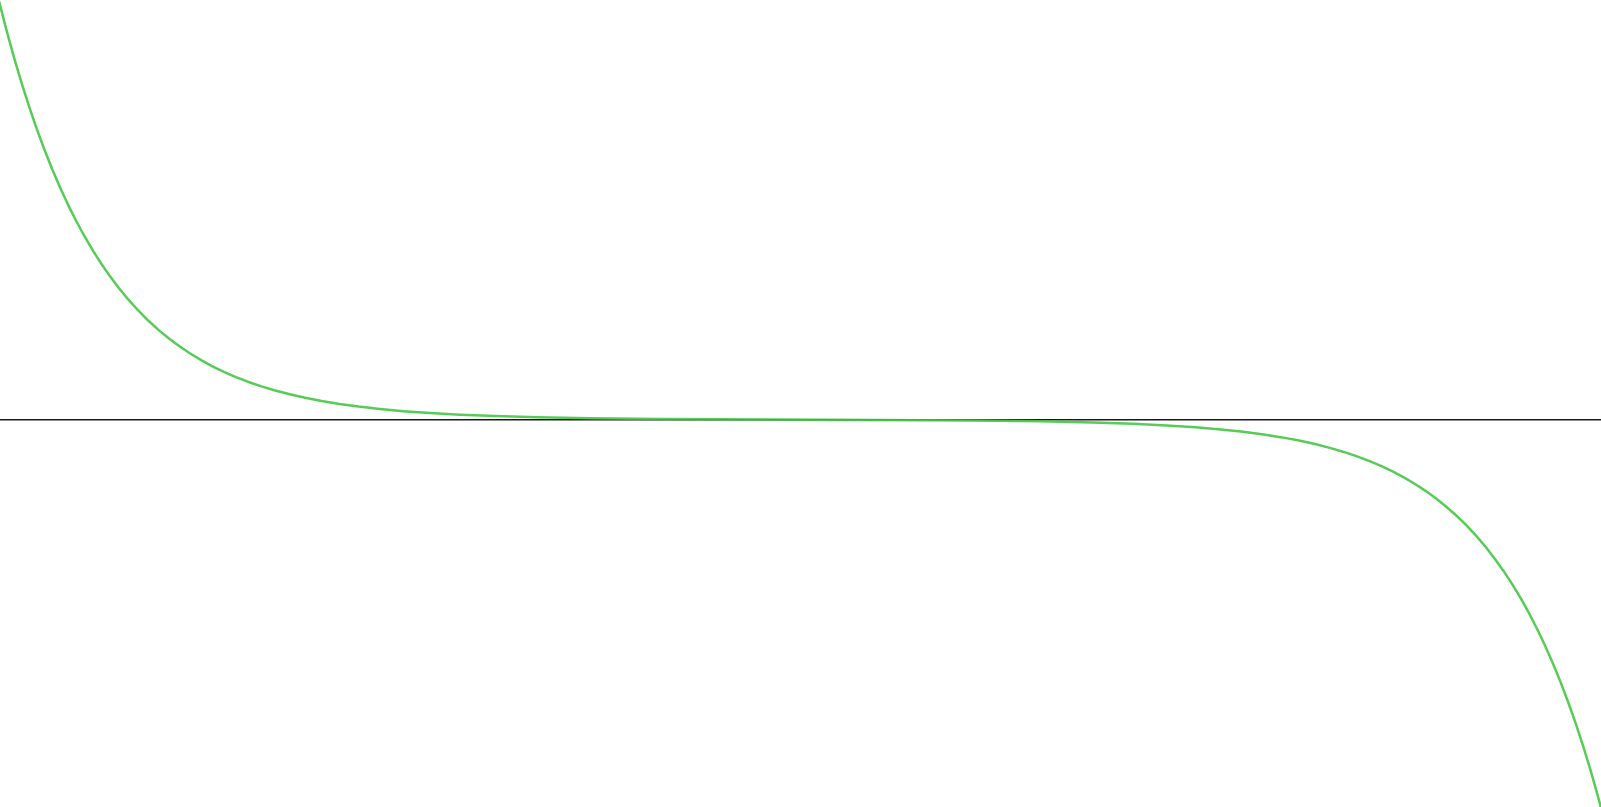
\includegraphics[width=0.5\linewidth]{../pic/3302/19.png}
		\end{center}
	\item if $\frac{\phi"}{\phi} = -k^2 \implies \phi = Ae^{ikx} +Be^{-ikx}$ :
		\begin{center}
			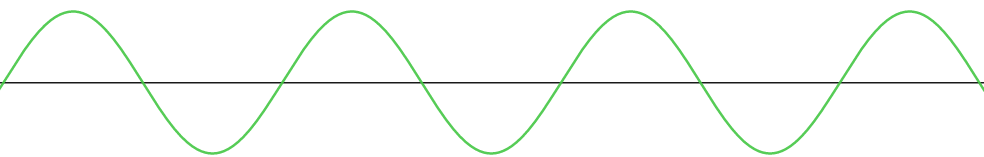
\includegraphics[width=0.5\linewidth]{../pic/3302/20.png}
		\end{center}
\end{itemize}
 $\begin{cases}
	\text{ if }E-U < 0 \implies \frac{\phi"}{\phi}>0 \implies \text{ solution : } Ae^{kx} + Be^{-kx}\\
	\text{ if }E-U > 0 \implies \frac{\phi"}{\phi}<0 \implies \text{ solution : } Ae^{ikx}+Be^{-ikx}
\end{cases} \implies $
\begin{center}
	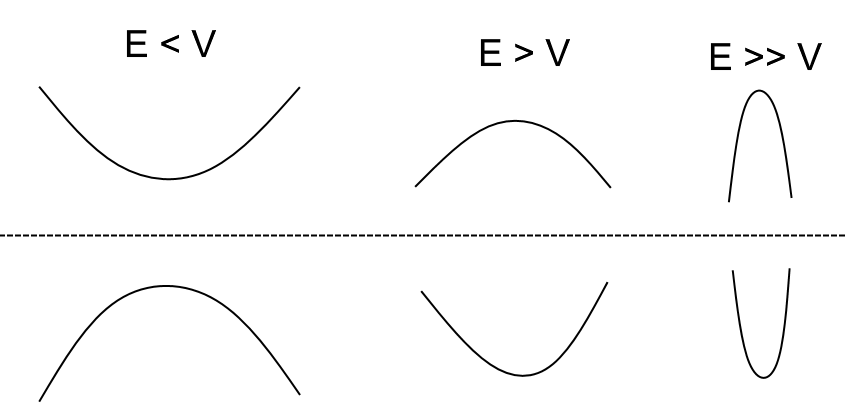
\includegraphics[width=0.5\linewidth]{../pic/3302/18.png}
\end{center}

\section{Stationary states}
Consider the state $\psi(x,t) = e^{-iwt}\phi_E(x)$ where $\phi_E(x)$ : energy eigenfunction.\\
$\psi(x,t)$ is called a stationary state because it's probability density independent of time.\\
The probability density at time t measuring the particle at position x is :\\
$\p(x,t) = |\psi(x,t)|^2 = |\phi_E(x)|$ \underline{Independent of time }.\\
So, if we happen to know that our state is in an n energy eigenfunction, then the probability density for finding the particle at any given position does not change in time.\\
Consequence :
\begin{itemize}
	\item $\moyenne{x}_{t} = \int dx \p(x,t)x = \int dx |\phi_E(x)|^2x = \moyenne{x}_{t=0} $
	\item Having solved the Schrödinger equation once for energy eigenstate allows us to solve it for general superposition:
	      \[\psi(x,0) = \sum_nC_n\phi_n(x)\implies \psi(x,t)= \sum_nC_ne^{-iw_nt}\phi_n(x)\]
	      That mean that we can take an arbitrary initial condition ($\psi(x,0) = \sum_n C_n\phi_{E_n}(x)$) and compute the full solution of the Schrödinger equation($ \psi(x,t)= \sum_nC_ne^{-iw_nt}\phi_n(x)$).\\
	      All we have to do is figure out what these coefficients $C_n$ are.\\
	      Meanwhile, these coefficients are corresponded to the probability that we measure the energy to be equal to the corresponding energy $E_n$:$\p(A=a) = |C_a|^2$
\end{itemize}
\section{Free Particle}
$\hat{E} = \frac{\hat{p}^2}{2m} = -\frac{\hbar^2}{2m}\partial_x^2$ \\
$\hat{E}\phi_E = E\phi_E \Leftrightarrow \frac{-\hbar^2}{2m}\phi"(x) = E\phi(x) \\
	\phi"(x) + \frac{2mE}{\hbar^2}\phi(x) = 0; k^2 = \frac{2mE}{\hbar^2}$\\
The general solution is : $\phi_E(x) = Ae^{ikx} + Be^{-ikx};E =\frac{\hbar^2k^2}{2m}$
\section{Particle in the Box}
\begin{center}
	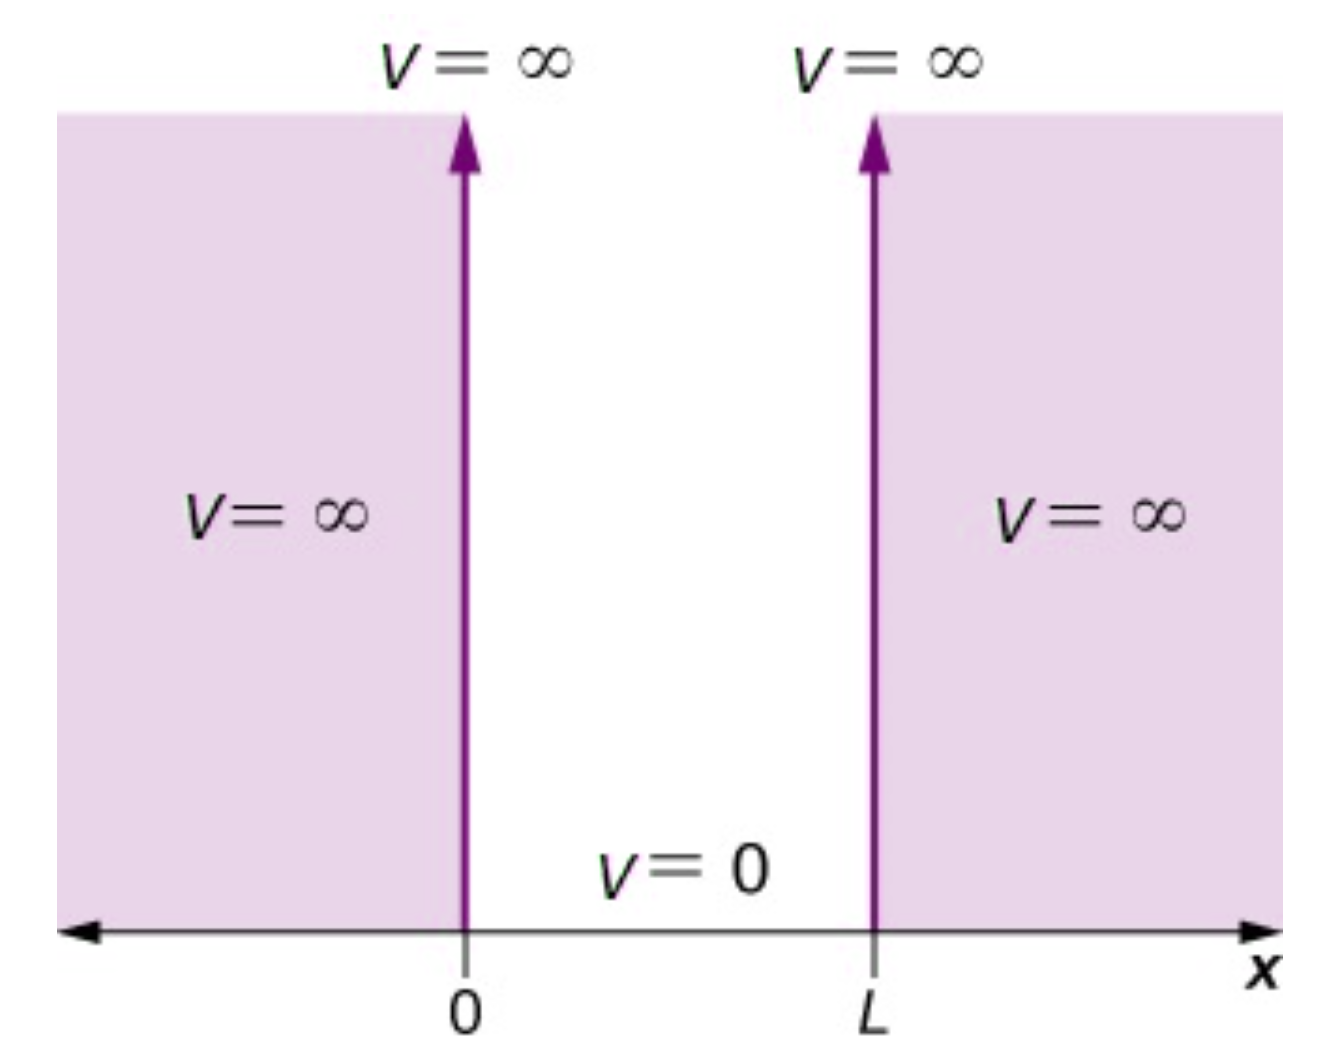
\includegraphics[width=0.5\linewidth]{../pic/3302/15.png}
\end{center}
$\p(x<0 , x> L) = 0 \implies \psi(x)= 0 $ and at $x=0,x=L$.\\
Inside the box the equation is as the free particle, so the general solution is :\\
$\phi_E = De^{ikx} + Ce^{-ikx} =\alpha\cos(kx) + \beta\sin(kx)$ \\
$x =0 \implies \alpha = 0\\
	x = L \implies kx = n\pi  \implies k_n = \frac{n\pi}{L}$  where $n $ integer $\geq 1$.\\
After normalization : $\phi_E = \sqrt{\frac{2}{L}}\sin(k_nx);E_n = \frac{\hbar^2k_n}{2m} = \frac{\hbar^2\pi^2n^2}{2mL^2}$ \\
With the superposition postulate, we can write :\\
$\psi(x,0) = \sum_n \phi_n(x)C_n \implies \boxed{\psi(x,t) = \sum_n\phi_n(x)e^{-i\frac{\hbar k_n^2}{2m}t}C_n}$
\begin{center}

	\begin{minipage}{0.3\linewidth}
		$\psi(x):$ \\
		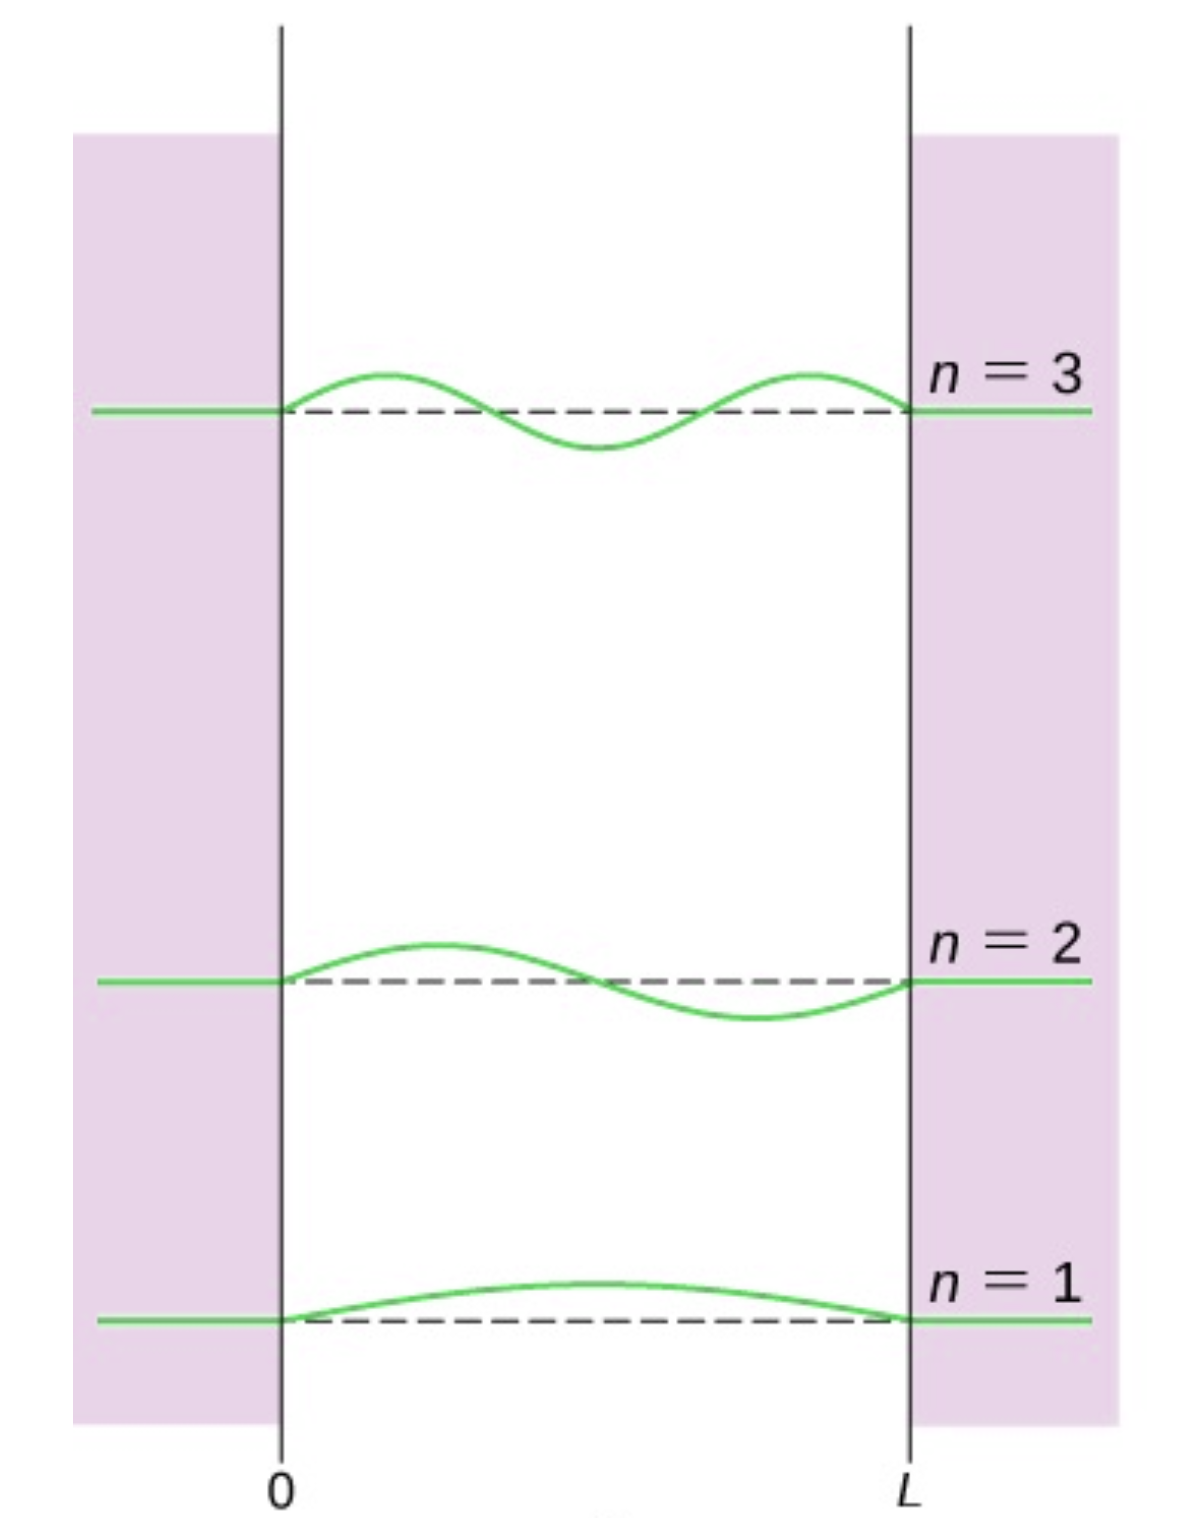
\includegraphics[width=\linewidth]{../pic/3302/16.png}
	\end{minipage}
	\begin{minipage}{0.5\linewidth}
		$\p(x)$:\\
		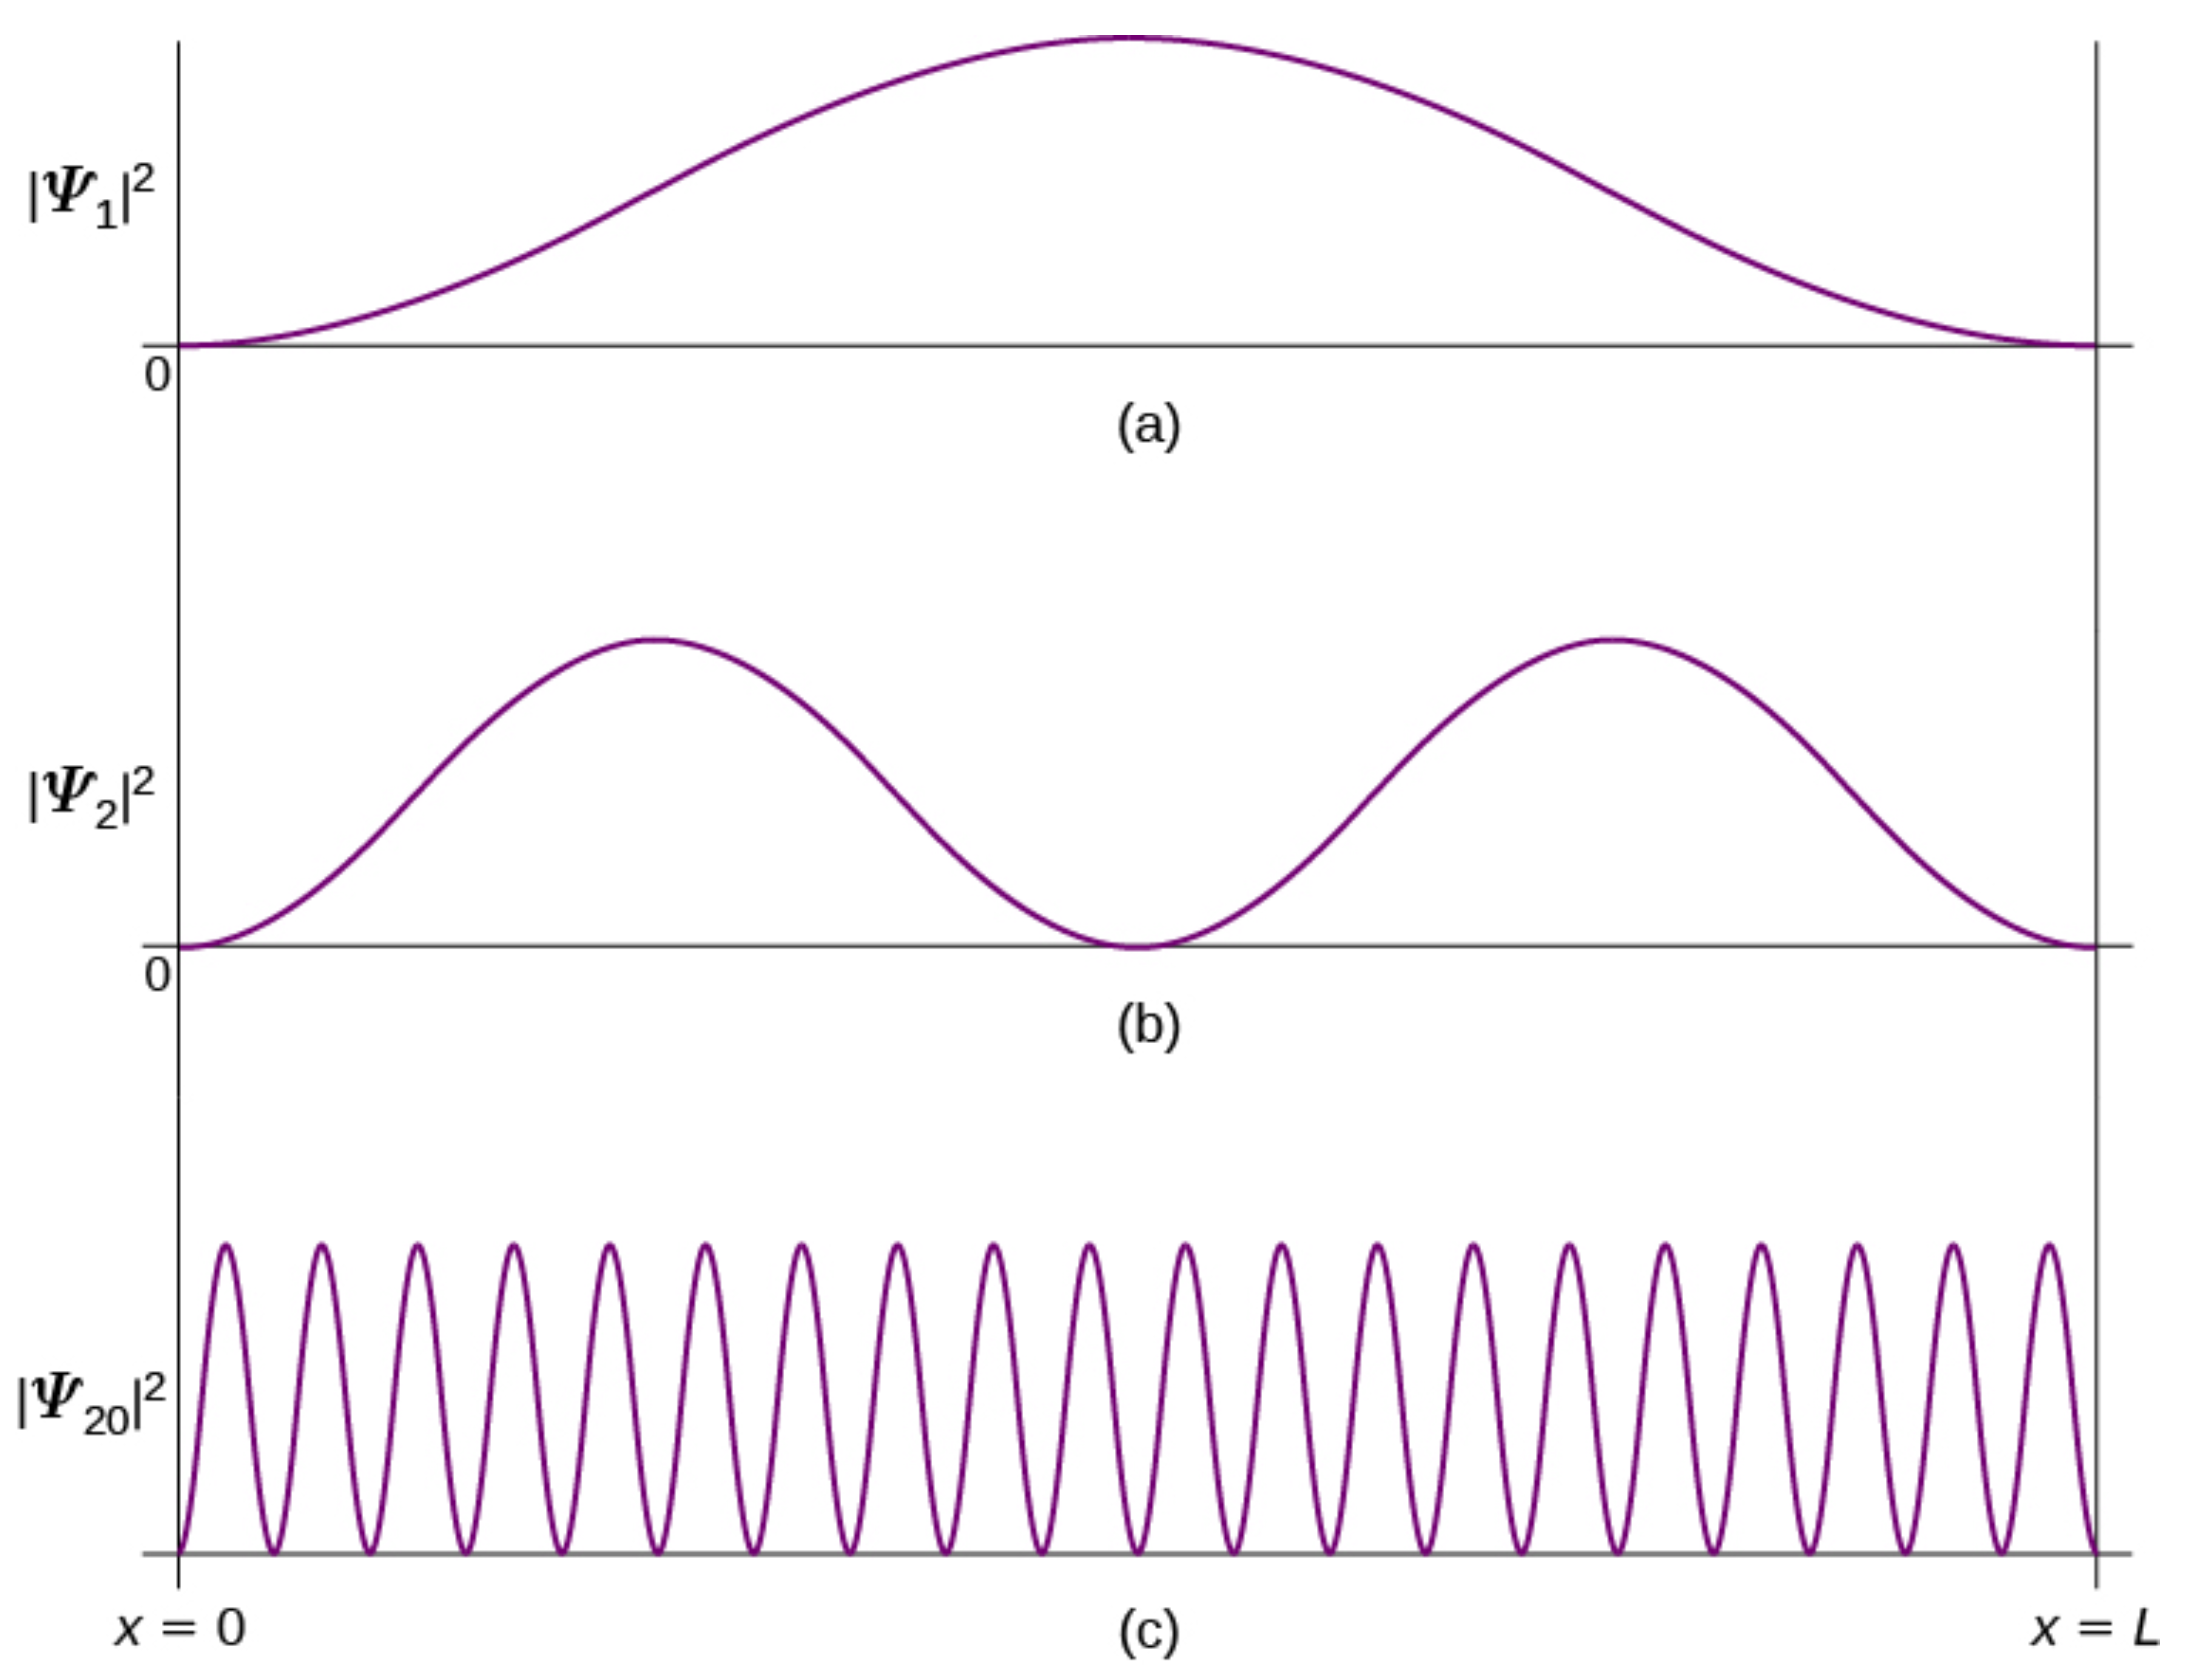
\includegraphics[width=\linewidth]{../pic/3302/17.png}
	\end{minipage}

\end{center}
\section{Harmonic Oscillator}
\subsection{Brute Force}
The total energy $E$ of a particle of mass m moving in one dimension under the action of a restoring force $F = -kx,k>0$, is usually written as :
\[E = \underbrace{\frac{1}{2}mv^2}_\text{kinetic energy} + \underbrace{\frac{1}{2}kx^2}_\text{potential energy}\]
The potential is quadratic in x. $\implies w = \sqrt{\frac{k}{m}} \to k = mw^2$\\
We can rewrite E as follows :
\[E = \frac{p^2}{2m} + \frac{1}{2}mw^2x^2\]
The Schrödinger equation :
\[ -\frac{\hbar^2}{2m}\frac{d^2\phi(x)}{dx^2}+\frac{1}{2}mw^2x^2\phi(x) + E\phi(x) \]
\begin{itemize}
	\item Clean the equation of dimensional constants\\
	      We multiply the equation by $(\frac{2}{\hbar w})$
	      \[ \underbrace{\frac{-\hbar}{mw}\frac{d^2}{dx^2}}_\text{unite free}\phi + \underbrace{\frac{mw}{\hbar}x^2}_\text{unit free}\phi = \underbrace{\frac{2E}{\hbar w}}_\text{unit free}\phi  \]
	      We define a unit free energy $\varepsilon = \frac{2E}{\hbar w}$\\
	      We set $x = au$ ($u$ unit free , $[a] = L$) then we have $\frac{d}{dx} = \frac{1}{a}\frac{d}{dx};\frac{d^2}{dx^2} = \frac{1}{a^2}\frac{d^2}{dx^2}$\\
	      The equation now is :
	      \[\frac{d^2\phi}{du^2} = (u^2-\varepsilon)\phi\]
	\item Now how this solution look as u goes to infinity the equation became $\boxed{\psi" = u^2\psi}$\\
	      We will try the solution :$\psi = u^ke^{\alpha \frac{u^2}{2}}$ where $\alpha$ is a number then :
	      \[\psi' = \alpha u u^k e^{\alpha \frac{u^2}{2}} + ku^{k-1}e^{\alpha \frac{u^2}{2}}\]
	      and :
	      \begin{align*}
		      \psi"  & = (\alpha u^2)u^k e^{\alpha \frac{u^2}{2}} + ...  = \alpha^2u^2u^ke^{\alpha\frac{u^2}{2}}[1+ \frac{2k+1}{\alpha}\frac{1}{u^2}+\frac{k(k-1)}{\alpha^2}\frac{1}{u^4}] \\
		      \psi " & = \alpha^2u^2\psi[1+\frac{2k+1}{\alpha}\frac{1}{u^2} + ...]
	      \end{align*}
	      When $u$ goes to infinity, our solution works because $[1+\frac{2k+1}{\alpha}\frac{1}{u^2}+...]$ is negligible.\\
	      So we get a number $\alpha$ times $u^2$ (it is the equation that we are trying to solve)
	      \[ \psi "  = \alpha^2u^2\psi \Longleftrightarrow \psi" = u^2\psi\]
	      and therefore $\alpha^2 = 1\implies \alpha = \pm 1$ \\
	      So we expect as u goes to infinity :\\
	      $\psi(u) = Au^ke^{-\frac{u^2}{2}} + Bu^ke^{+\frac{u^2}{2}}\begin{cases}
			      Au^ke^{-\frac{u^2}{2}} : \text{Converge at infinity } \\
			      Bu^ke^{+\frac{u^2}{2}} : \text{Diverge at infinity}
		      \end{cases} \implies \boxed{\psi(u) = Au^ke^{-\frac{u^2}{2}}}$
	\item Write $\psi(u) = h(u)e^{-\frac{u^2}{2}}$ to simplify the solution.\\
	      because the exponential equation has been taken care of, now we can find a simple solution for $h(u)$.\\
	      We substitute in the differential equation, and we obtain :
	      \[\frac{d^2 h}{du^2}-2u\frac{dh}{du}+(\varepsilon-1)h = 0\]
	      The way we solve this equation is by power series expansion:\\
	      $h(u) = \sum^\infty_{j=0} a_ju^j\implies \frac{dh(u)}{du} = \sum_{j=0}^\infty ja_ju^{j-1} \implies \frac{d^2 h}{du^2} = \sum^\infty_{j=0}j(j-1)a_ju^{j-2} = \sum^\infty_{j=2}j(j-1)a_ju^{j-2}$\\
	      let j = j'+2 $ \implies \frac{d^2 h}{du^2} =\sum^\infty_{j'=0} (j'+2)(j'+1)a_{j'+2}u^{j'} = \sum^{\infty}_{j=0}(j+2)(j+1)a_{j+2}u^j$\\
	      Replace in the equation : \\
	      $ 0 = \sum^\infty_{j=0}((j+2)(j+1)a_{j+2}-2ja_j +(\varepsilon -1)a_j )u^j = \sum^{\infty}_{j=0}((j+2)(j+1)a_{j+2} -(2j+1-\varepsilon)a_j )u^j$\\
	      $\implies \boxed{a_{j+2} = \frac{2j+1-\varepsilon}{(j+2)(j+1)}a_j}$ (That solves for $a_{j+2}$ in terms of $a_j$) \\
	      So the solution is determined by the value of the two constant $a_0$ and $a_1$, that's what you expect from a second order differential equation (The value of the function($a_0$) and it's derivative ($a_1$) at a point) \\
	      The solution is fixed by given $\underbrace{a_0}_\text{even solutions},\underbrace{a_1}_\text{odd solution}$ corresponding to h(0),h'(0).\\
	      But the series must terminate, so to terminate $2j+1-\varepsilon=0$ this will make $a_{j+2} = 0$.\\
	      Now let'us call $j=n$ , we have $2n+1-\varepsilon_n = 0$ and $h(u) = a_nu^n + ...$ \\
	      We recall $\varepsilon_n = \frac{E_n}{\frac{\hbar w}{2}} = 2n+1 \implies E_n = \frac{\hbar w}{2}(2n+1) = \hbar w(n+\frac{1}{2}) $\\
	\item Actually, $h(u)_n $ is what we call the Hermite function of $u_n$ : $h(u)_n = H_n(u) = 2^nu^n+O(u^{n-2})$\\
	      The equation become :
	      $\frac{d^2H_n}{du^2}-2u\frac{dH_n}{du}+2nH_n = 0$\\
	      The whole solution : $\psi_n = H_n(u)e^{\frac{-u^2}{2}} \implies \boxed{\psi_n(x) = H_n(\frac{x}{a})e^{-\frac{x^2}{2a^2}}}$
\end{itemize}


\subsection{Operator Method}
The energy operator for the harmonic oscillator :
\[ \hat{E} = \frac{\hat{p}^2}{2m}+\frac{mw^2}{2}\hat{x}^2 \]
Dimension analysis, those are the parameter that matter:\\
The parameters that could possibly appear during the answer :$\begin{cases}
		\hbar [px] \\
		m [m]      \\
		w [\frac{1}{T}]
	\end{cases}\implies \begin{cases}
		[hmw] = [p]^2 \\
		[\frac{\hbar}{mw}] = [x]^2
	\end{cases}$\\
So we define $\begin{cases}
		x_0 = \sqrt{\frac{2\hbar}{mw}} \\
		p_0 = \sqrt{2\hbar m w}        \\
		x_0p_0=2\hbar
	\end{cases}$ \\
Now we can rewrite the energy operator as $\hat{E} = \hbar w [\frac{\hat{p}^2}{p_0^2}+\frac{\hat{x}^2}{x_0^2}]$\\
We are interested in the energy operator, and it is a  sum of squares, so we will factor it:\\
\push{For two complexe numbers  $c^2 + d^2 = (c-id)(c+id)$\\
	Is that true for operaters ? le us try it \\
	$(\frac{\hat{x}}{x_0}-i\frac{\hat{p}}{p_0})(\frac{\hat{x}}{x_0}+i\frac{\hat{p}}{p_0}) = \frac{\hat{x}^2}{x_0^2} + \frac{\hat{p}^2}{p_0^2} + \frac{i}{2k}[\hat{x},\hat{p}]$\\
	the commutator $[\hat{x},\hat{p}] = i\hbar \implies (\frac{\hat{x}}{x_0}-i\frac{\hat{p}}{p_0})(\frac{\hat{x}}{x_0}+i\frac{\hat{p}}{p_0})  = \frac{\hat{x^2}}{x_0^2} + \frac{\hat{p}^2}{p_0^2} - \frac{1}{2}$}
Then we can write the energy operator $\hat{E} = \hbar w [\frac{\hat{p}^2}{p_0^2}+\frac{\hat{x}^2}{x_0^2}] $ as:$\hat{E}= hw((\frac{\hat{x}}{x_0}-i\frac{\hat{p}}{p_0})(\frac{\hat{x}}{x_0}+i\frac{\hat{p}}{p_0}) +\frac{1}{2})$\\
Consider the following :$\hat{a} = (\frac{\hat{x}}{x_0} + i \frac{\hat{p}}{p_0}) , (\hat{a})\transpose =(\frac{\hat{x}}{x_0} - i \frac{\hat{p}}{p_0}) $\\
Now we can write $\hat{E}$ as :
\[\boxed{\hat{E} = \hbar w(\hat{a}\transpose\hat{a}+\frac{1}{2})}\]
$\hat{a}\transpose \not = \hat{a} \implies \hat{a}$ is not hermitian $\implies \hat{a}$ not observable operator. \\
$\hat{a}$ and $\hat{a}\adjoint$ satisfy the commutation relation:
\[[\hat{a},\hat{a}\adjoint] = [(\frac{\hat{x}}{x_0}+i\frac{\hat{p}}{p_0}),(\frac{\hat{x}}{x_0}-i\frac{\hat{p}}{p_0})] = \frac{-i}{2\hbar}[x,p] + \frac{i}{2\hbar}[p,x] = \frac{1}{2} + \frac{1}{2} = 1\implies \begin{cases}
		\boxed{[a,a\adjoint] = 1} \\
		\boxed{[a\adjoint,a] = -1}
	\end{cases}\]
$[\hat{E},\hat{a}]=\hbar w(\hat{a}\transpose\hat{a} + \frac{1}{2})(\hat{a})-\hbar w(\hat{a})(\hat{a}\transpose\hat{a} + \frac{1}{2})=\hbar w[a\adjoint,a]=\hbar w (a\adjoint a a - a a\adjoint a)\\
	= \hbar w(a\adjoint a - a a\adjoint)a=-\hbar w a\implies \begin{cases}\boxed{[\hat{E},\hat{a}] = -\hat{a}\hbar w }\\ \boxed{[E,a\adjoint] = + a\adjoint \hbar w}\end{cases}$\\
Suppose that we already happened to have access to an eigenfunction of the energy operator : $\hat{E} \phi_E = E \phi_E $.\\
Now consider a new state $\psi$, which is equal to : $\psi = \hat{a}\phi_E$\\
\[\hat{E}\psi = \hat{E}\hat{a}\phi_E = (\hat{E}\hat{a}-\hat{a}\hat{E} + \hat{a}\hat{E})\phi_E= ([\hat{E},\hat{a}] + a \hat{E})\phi_E =(-\hbar w \hat{a} + E \hat{a})\phi_E = (E -\hbar w )\underbrace{\hat{a}\phi_E}_\psi\]
\[\boxed{\hat{E} =(E -\hbar w )\hat{a}\psi}\]
\begin{center}
	(Note : if we have operator A, B and the state F we can write $\hat{A}\hat{B}f = ([\hat{A},\hat{B}]+BA)f$, with this way we can act A on f directly without B,  but we have to know the commutator of $[\hat{A},\hat{B}]$)
\end{center}
So if we have a state with energy E, and we act on it with the operator $\hat{a}$ ,we get new state $\psi$ which is also an eigenstate of the energy operator but with a different energy eigenvalue (it decreased by $\hbar w$).\\
That mean if we have $\hat{E}\phi_E = E \phi_E, \hat{a}\phi_E $ has energy :$ E-\hbar w \implies \psi = \phi_{E-\hbar w}$ \\
Now let us call $\begin{cases}
		\hat{a}:\text{ the lowering operator}       \\
		\hat{a}\adjoint:\text{the raising operator} \\
	\end{cases}$\\
\begin{center}
	By applying the lowering operator and the raising operator, we get a set of energy eigenstate evenly spaced by $\hbar w$ because of commutation relation $[\hat{E},\hat{a}]$.
\end{center}
So what about the \underline{WAVE FUNCTION} ?
\begin{itemize}
	\item We know that $\hat{a}\phi_0(x) = 0$ , $\phi_0$ is the ground state.\\
	      (Note that the ground state is the state just above the 0 energy)
	\item And we know that the lowering operator $\hat{a} = (\frac{\hat{x}}{x_0} + i \frac{\hat{p}}{p_0})$
	\item if we apply the lowering operator on the ground state we will get the energy below that state which is 0.\\
	      $ \hat{a}\phi_0=\boxed{(\partial_x + \frac{2}{x_0^2}x)\phi_0 = 0}$ \\
	\item This differential equation have this form of solution, $\phi_0 = C e^{-\frac{x^2}{x_0^2}}$
	\item we can get the set of all states by applying the lowering-raising operators : \\
	      $\phi_1 = \hat{a}\adjoint\phi_0 = N(\partial_x - \frac{2}{x_0^2}x)\phi_0,\\
		      \phi_2 =N(\partial_x - \frac{2}{x_0^2}x)^2\phi_0,\\
		      \phi_3 =N(\partial_x - \frac{2}{x_0^2}x)^3\phi_0,\\
		      ...$ \\
	      N is a constant up to some normalization.
\end{itemize}
\begin{center}
	The upshot of all this is that we've derived that without ever solving the differential equation the spectrum just from this commutation relation $[\hat{E},\hat{a}] = -\hat{a}\hbar w$
\end{center}
\section{Finite Potential Well}
	We want to find the energy eigenstate of the finite well, because we want to study the time evolution,and the easiest way to study time evolution is to expand an energy eigenstate $\phi_E$
	$E\phi_E(x) = \frac{-\hbar^2}{2m}\phi_E"(x)+V(x)\phi(x) $\\
	$\boxed{\phi"(x) = \frac{2m}{\hbar^2}(V(x)-  E)\phi(x)}$\\
	We expect the Energie state be discrete  then if the energy greater than the potential everywhere the energies will be continuous.\\
	Our boundary conditions : 
	\begin{itemize}
		\item Normalizable infinity. the solution should be vanishing far away.
		\item The wave function should be everywhere smooth.
		\item Continuity of $\phi_E$ 
	\end{itemize}
	Note : \\ 
	\begin{center}
		\begin{minipage}{0.32\linewidth}
			if $V(x)$ continues : 
		\begin{itemize}
			\item $\phi"$ continues
			\item $\phi'$ continues
			\item $\phi$ continues
		\end{itemize}
		\end{minipage}
		\begin{minipage}{0.32\linewidth}
			if $V(x)$ has step :
		\begin{itemize}
			\item $\phi"$ discontinues
			\item $\phi'$ continues
			\item $\phi$ continues
		\end{itemize}
		\end{minipage}
		\begin{minipage}{0.32\linewidth}
			if $V(x)$ has $\delta(x)$ :
			\begin{itemize}
				\item  $\phi"$ like $\delta(x)$
				\item $\phi'$ step 
				\item $\phi$ continuous
			\end{itemize}
		\end{minipage}
	\end{center}
	Bound state : a quantum bound state it's an energy eigenstate such that the probability falls off exponentially as we go far away from wherever we think it is an interesting point, it is a state is just a state which  exponentially localized.\\
	if $E > V(x) \implies \phi" = -k^2\phi \implies $ oscillator\\
	if $E < V(x) \implies \phi" =  + \alpha^2\phi \implies$ exp ; $k^2 = \frac{2m}{\hbar^2}(E-V);\alpha^2 = \frac{2m}{\hbar^2}(V-E)$\\
	\begin{itemize}
		\item General Solution :$\phi_E(x) = \begin{cases}
			\rom{2} : A\cos(kx) + B\sin(kx) \\
			\rom{1} : Ce^{\alpha x} + D e^{-\alpha x}\\
			\rom{3}:  \xi 	e^{\alpha x} + F e^{-\alpha x}
		\end{cases}$
		\item Normalizable : 
		$\begin{cases}
			\phi(x\to -\infty) = 0 \implies D = 0\\
			\phi(x\to + \infty) = 0 \implies \xi = 0
		\end{cases}$
		\item We can take advantage from the parity of well : \\
		the system is either symmetric (even) or anti-symmetric (odd).\\
		if the system is even $\implies B = 0 ; C =F$ \\
		if the system is antisymmetric $\implies A = 0 ; C = -F $\\
	
		For now we are working with the even solution so the system become : 
		\item Left boundary condition x = 0: 
		$\begin{cases}
			\phi \text{contiues} \\
			\phi' \text{continuies}
		\end{cases}$
		\item Right boundary condition x = L : 
		$\begin{cases}
			\phi \text{contiues} \implies \phi = A \cos(KL) = C e^{-\alpha L} \implies C = A\cos(kL)e^{\alpha L}\\
			\phi' \text{continuies} \phi' = -Ak\sin(KL) = - \alpha Ce^{-\alpha L} \implies C = A \frac{k}{\alpha}\sin(kL)e^{\alpha L}
		\end{cases}$
		So if we impose the continuity condition for the wave function we can find a solution.\\
		Similarly if we impose only the continuity condition for the derivative we can find a solution for arbitrary values of the energy . \\
		But in order to find a solution where the wave function and its derivative are both continuous :
		It can't be true that the energy takes just any value because it would tell that c takes two different values  
		\begin{center}
			SO there is a consistency condition For what values of energy or equivalently values of $KL$ are these two equation are equal to the same thing
		\end{center}
		We want both of these equation to be true : \\
		so we can divide the second equation by the first one $\implies    k\tan(kL) = \alpha$ we can multiply by L (to make the equation dimensionless)$\implies Lk\tan(kL) = \alpha L$ condition on the energy .\\

		The boundary condition on the left well give the same expression $ k\tan(kL) = \alpha$

		\item Graphical Solution $KL = Z ; \alpha L = y$\\
			$z^2 + y^2 = \frac{2m}{\hbar^2}V_0 = \mathbb{R}_0^2$ so this is a equation of a circle . \\
			So we have the two equation $\begin{cases}
				z\tan(z) = y : \text{\textcolor{black}{black color}}\\
				z^2 + y^2 = \mathbb{R}_0^2 : \text{\textcolor{red}{red color}}
			\end{cases}$
			\begin{center}
				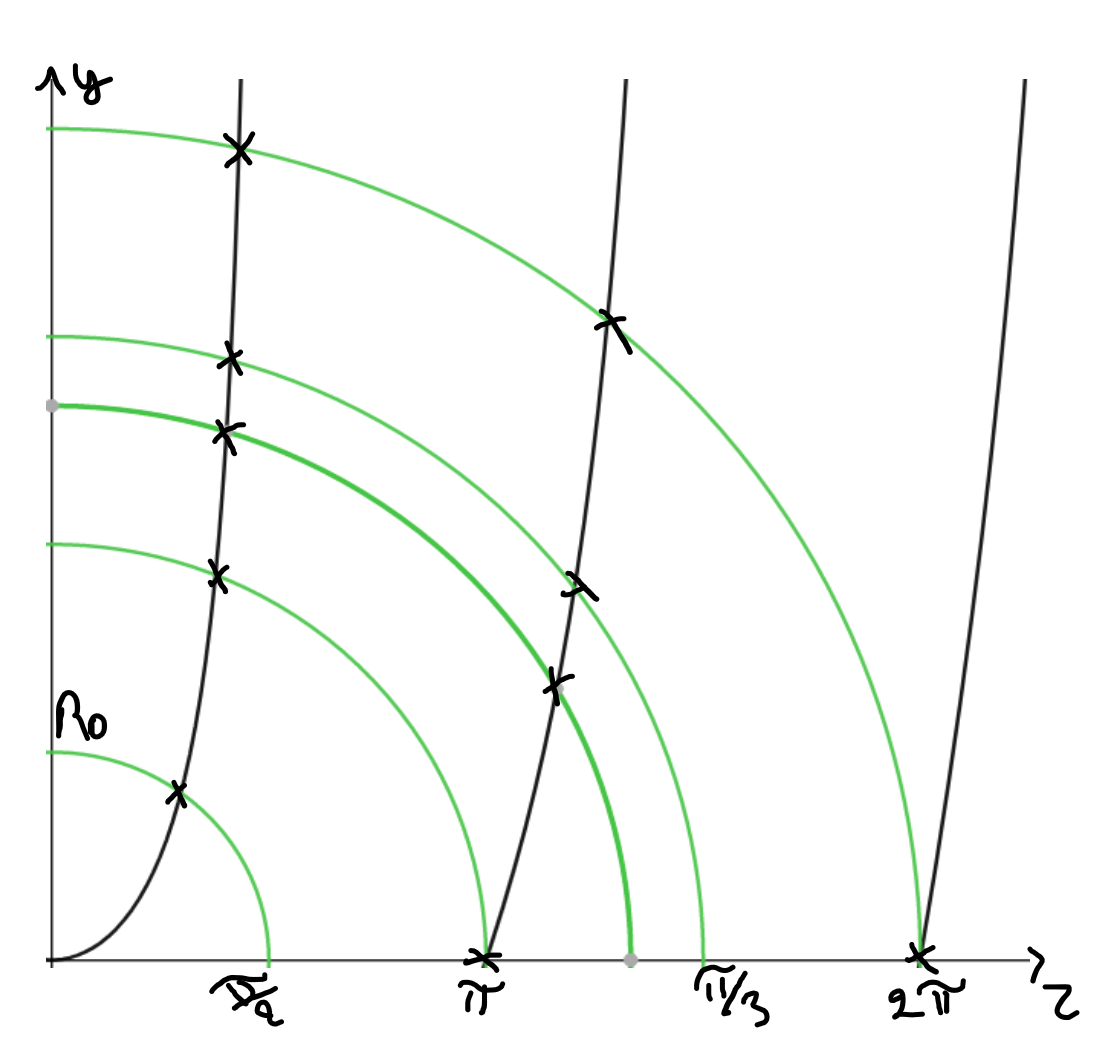
\includegraphics[width=0.5\linewidth]{../pic/3302/21.png}
			\end{center}
			the intersection red - black point are solution , a bound state
			$L$ larger $\mathbb{R}$ get larger , we got more and more state
			$V $ larger $\mathbb{R}$ get larger the number of states increase (there more point where this circle intersect this point.)\\
			$V$ get less $\mathbb{R}$ get less but we never loose a bound state , there is no circle so small that it doesn't intersect with this curve .\\
			$\implies $ at 1D, finite well potential there is always at least one  bound state .

			Now For $\mathbb{R}_0 = \pi $, this "bound state"  at "threshold" $E = V$ , have exceedingly long tails, and they're just barely bound.

			Now if $V $ is so deep $\implies$ infinite well;
			\begin{center}
				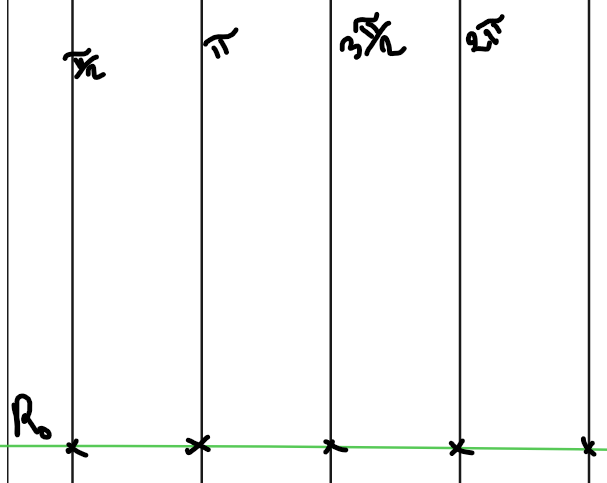
\includegraphics[width=0.5\linewidth]{../pic/3302/22.png}
			\end{center}
			z became : $z = \frac{2n+1}{2}\pi \implies k = \frac{2n+1}{2L}\pi$
			those value of k are almost the same value for the infinite well , instead of $\frac{2n+1}{2L}$ it should be $\frac{n+1}{2L}$.\\
			we seem to be missing about half of the energy eigenvalues, but those are only the even one.\\
			so for the odd we expect : $k = \frac{2n+2}{2L}\pi$

			For the following potential : $ V =- V_0\delta(x) $ \\
			$\phi_E(x) = \begin{cases}
				Ae^{\alpha x} + Be^{-\alpha x}  ; x< 0 \\
				Ce^{\alpha x} + A e^{-\alpha x} ; x>0
			\end{cases}$
	\end{itemize}
\end{document}